% Options for packages loaded elsewhere
\PassOptionsToPackage{unicode}{hyperref}
\PassOptionsToPackage{hyphens}{url}
\PassOptionsToPackage{dvipsnames,svgnames,x11names}{xcolor}
%
\documentclass[
  a4paper,
  table]{article}

\usepackage{amsmath,amssymb}
\usepackage{iftex}
\ifPDFTeX
  \usepackage[T1]{fontenc}
  \usepackage[utf8]{inputenc}
  \usepackage{textcomp} % provide euro and other symbols
\else % if luatex or xetex
  \usepackage{unicode-math}
  \defaultfontfeatures{Scale=MatchLowercase}
  \defaultfontfeatures[\rmfamily]{Ligatures=TeX,Scale=1}
\fi
\usepackage{lmodern}
\ifPDFTeX\else  
    % xetex/luatex font selection
\fi
% Use upquote if available, for straight quotes in verbatim environments
\IfFileExists{upquote.sty}{\usepackage{upquote}}{}
\IfFileExists{microtype.sty}{% use microtype if available
  \usepackage[]{microtype}
  \UseMicrotypeSet[protrusion]{basicmath} % disable protrusion for tt fonts
}{}
\makeatletter
\@ifundefined{KOMAClassName}{% if non-KOMA class
  \IfFileExists{parskip.sty}{%
    \usepackage{parskip}
  }{% else
    \setlength{\parindent}{0pt}
    \setlength{\parskip}{6pt plus 2pt minus 1pt}}
}{% if KOMA class
  \KOMAoptions{parskip=half}}
\makeatother
\usepackage{xcolor}
\usepackage[margin=2.5cm]{geometry}
\setlength{\emergencystretch}{3em} % prevent overfull lines
\setcounter{secnumdepth}{5}
% Make \paragraph and \subparagraph free-standing
\makeatletter
\ifx\paragraph\undefined\else
  \let\oldparagraph\paragraph
  \renewcommand{\paragraph}{
    \@ifstar
      \xxxParagraphStar
      \xxxParagraphNoStar
  }
  \newcommand{\xxxParagraphStar}[1]{\oldparagraph*{#1}\mbox{}}
  \newcommand{\xxxParagraphNoStar}[1]{\oldparagraph{#1}\mbox{}}
\fi
\ifx\subparagraph\undefined\else
  \let\oldsubparagraph\subparagraph
  \renewcommand{\subparagraph}{
    \@ifstar
      \xxxSubParagraphStar
      \xxxSubParagraphNoStar
  }
  \newcommand{\xxxSubParagraphStar}[1]{\oldsubparagraph*{#1}\mbox{}}
  \newcommand{\xxxSubParagraphNoStar}[1]{\oldsubparagraph{#1}\mbox{}}
\fi
\makeatother


\providecommand{\tightlist}{%
  \setlength{\itemsep}{0pt}\setlength{\parskip}{0pt}}\usepackage{longtable,booktabs,array}
\usepackage{calc} % for calculating minipage widths
% Correct order of tables after \paragraph or \subparagraph
\usepackage{etoolbox}
\makeatletter
\patchcmd\longtable{\par}{\if@noskipsec\mbox{}\fi\par}{}{}
\makeatother
% Allow footnotes in longtable head/foot
\IfFileExists{footnotehyper.sty}{\usepackage{footnotehyper}}{\usepackage{footnote}}
\makesavenoteenv{longtable}
\usepackage{graphicx}
\makeatletter
\newsavebox\pandoc@box
\newcommand*\pandocbounded[1]{% scales image to fit in text height/width
  \sbox\pandoc@box{#1}%
  \Gscale@div\@tempa{\textheight}{\dimexpr\ht\pandoc@box+\dp\pandoc@box\relax}%
  \Gscale@div\@tempb{\linewidth}{\wd\pandoc@box}%
  \ifdim\@tempb\p@<\@tempa\p@\let\@tempa\@tempb\fi% select the smaller of both
  \ifdim\@tempa\p@<\p@\scalebox{\@tempa}{\usebox\pandoc@box}%
  \else\usebox{\pandoc@box}%
  \fi%
}
% Set default figure placement to htbp
\def\fps@figure{htbp}
\makeatother

% Front page values. Edit here, nothing else needs to change for the title page.

\newcommand\reporttitle{Intrusion Detection Threat Report}

\newcommand\reportsubtitle{
JM2030 - Cybersecurity \\ \textbf{Intrusion Detection Report}
}

\newcommand\groupnumber{
\textbf{Group xx}
}

% One line per author: Name & Student number \\
\newcommand\reportauthors{
Rick de Rijk & 0000000 \\
Name Surname & 0000000 \\
}

\newcommand\grouptutor{
% Tutor: Name Surname
}

\newcommand\placeanddate{
's-Hertogenbosch, \today
}

% JADS colour (same as the TU/e logo colour in the original template)
\definecolor{JADS-colour}{RGB}{126,59,52}
\colorlet{Tue-red}{JADS-colour}
% Visual identity of the JADS report template, ported from General/Preamble.tex and
% General/Settings.tex of the original LaTeX template. Quarto already loads hyperref,
% xcolor, geometry, graphicx and booktabs, so those are not repeated here.

\usepackage{amsmath, amsthm, amssymb, amsfonts}
\usepackage{float}
\usepackage{caption}
\usepackage{subcaption}
\usepackage{tabularx}
\usepackage[nottoc,numbib]{tocbibind}
\usepackage{titlesec}
\usepackage{fancyhdr}
\usepackage[shortlabels]{enumitem}
\usepackage{lscape}
\usepackage{tikz}
\usetikzlibrary{positioning}
\usetikzlibrary{calc}
\usepackage{mlmodern}

% Coordinate helper used by the title page
\makeatletter
\newcommand{\gettikzxy}[3]{%
  \tikz@scan@one@point\pgfutil@firstofone#1\relax
  \edef#2{\the\pgf@x}%
  \edef#3{\the\pgf@y}%
}
\makeatother

\hypersetup{
    colorlinks=true,
    linkcolor=JADS-colour,
    urlcolor=JADS-colour,
    citecolor=JADS-colour
}
\urlstyle{same}

% Bullets
\renewcommand{\labelitemi}{\scriptsize\textcolor{JADS-colour}{$\blacksquare$}}
\renewcommand{\labelitemii}{\scriptsize\textcolor{JADS-colour}{$\square$}}
\renewcommand{\labelitemiii}{\textcolor{JADS-colour}{$\circ$}}
\renewcommand{\labelenumi}{\textbf{\textcolor{JADS-colour}{\arabic*.}}}
\renewcommand{\labelenumii}{\textbf{\textcolor{JADS-colour}{[\alph*]}}}
\renewcommand{\labelenumiii}{\textbf{\textcolor{JADS-colour}{\roman*.}}}

% Numbering tied to the section
\counterwithin{equation}{section}
\counterwithin{figure}{section}
\counterwithin{table}{section}

% Header and footer
\pagestyle{fancy}
\fancyhf{}
\lhead{
\includegraphics[height = 8pt]{template/figures/jads_logo.png}}
\rhead{\reporttitle}
\renewcommand{\headrulewidth}{0.4pt}
\renewcommand{\footrulewidth}{0.4pt}
\cfoot{Page \thepage}

% Section titles
\titleformat{\section}{\sffamily\color{JADS-colour}\Large\bfseries}{\thesection\enskip\color{gray}\textbar\enskip}{0cm}{}
\titleformat{\subsection}{\sffamily\color{JADS-colour}\large\bfseries}{\thesubsection\enskip\color{gray}\textbar\enskip}{0cm}{}
\titleformat{\subsubsection}{\sffamily\color{JADS-colour}\bfseries}{\thesubsubsection\enskip\color{gray}\textbar\enskip}{0cm}{}

% Captions
\DeclareCaptionFont{JADS-colour}{\color{JADS-colour}}
\captionsetup{labelfont={JADS-colour,bf}}

\setlength\parindent{0pt}
\setlength{\parskip}{0.6em}
\setcounter{tocdepth}{2}

% Alternating row shading for tables, in the house colour
\rowcolors{2}{JADS-colour!8}{white}
\makeatletter
\@ifpackageloaded{caption}{}{\usepackage{caption}}
\AtBeginDocument{%
\ifdefined\contentsname
  \renewcommand*\contentsname{Table of contents}
\else
  \newcommand\contentsname{Table of contents}
\fi
\ifdefined\listfigurename
  \renewcommand*\listfigurename{List of Figures}
\else
  \newcommand\listfigurename{List of Figures}
\fi
\ifdefined\listtablename
  \renewcommand*\listtablename{List of Tables}
\else
  \newcommand\listtablename{List of Tables}
\fi
\ifdefined\figurename
  \renewcommand*\figurename{Figure}
\else
  \newcommand\figurename{Figure}
\fi
\ifdefined\tablename
  \renewcommand*\tablename{Table}
\else
  \newcommand\tablename{Table}
\fi
}
\@ifpackageloaded{float}{}{\usepackage{float}}
\floatstyle{ruled}
\@ifundefined{c@chapter}{\newfloat{codelisting}{h}{lop}}{\newfloat{codelisting}{h}{lop}[chapter]}
\floatname{codelisting}{Listing}
\newcommand*\listoflistings{\listof{codelisting}{List of Listings}}
\makeatother
\makeatletter
\makeatother
\makeatletter
\@ifpackageloaded{caption}{}{\usepackage{caption}}
\@ifpackageloaded{subcaption}{}{\usepackage{subcaption}}
\makeatother

\usepackage[]{natbib}
\bibliographystyle{IEEEtranDOI}
\usepackage{bookmark}

\IfFileExists{xurl.sty}{\usepackage{xurl}}{} % add URL line breaks if available
\urlstyle{same} % disable monospaced font for URLs
\hypersetup{
  colorlinks=true,
  linkcolor={blue},
  filecolor={Maroon},
  citecolor={Blue},
  urlcolor={Blue},
  pdfcreator={LaTeX via pandoc}}


\author{}
\date{}

\begin{document}

\begin{titlepage}

\centering

\begin{tikzpicture}

\node[opacity=0.3,inner sep=0pt,remember picture,overlay] at (4.5,-0.5){
\includegraphics[width= 0.8 \textwidth]{template/figures/jads_logo_grey.png}};

\node[inner sep=0pt] (logo) at (0,0)
    {
\includegraphics[width=.25\textwidth]{template/figures/jads_logo.png}};

\node[text width = 0.5\textwidth, right = of logo](title){\sffamily\huge\reporttitle};

\node[text width = 0.5\textwidth, yshift = 0.75cm, below = of title](subtitle){\sffamily\Large \reportsubtitle};

\gettikzxy{(subtitle.south)}{\sffamily\subtitlex}{\subtitley}
\gettikzxy{(title.north)}{\titlex}{\titley}
\draw[line width=1mm, Tue-red]($(logo.east)!0.5!(title.west)$) +(0,\subtitley) -- +(0,\titley);

\end{tikzpicture}
\vspace{3cm}

\sffamily\groupnumber

\vspace{1em}

{\sffamily\large
\begin{tabular}{ll}
\textbf{Full Name} & \textbf{Student ID}\\
\hline
\reportauthors
\end{tabular}
}

\vspace{1em}
\sffamily \grouptutor

\tikz[remember picture,overlay]\node[anchor=south,inner sep=0pt] at (current page.south) {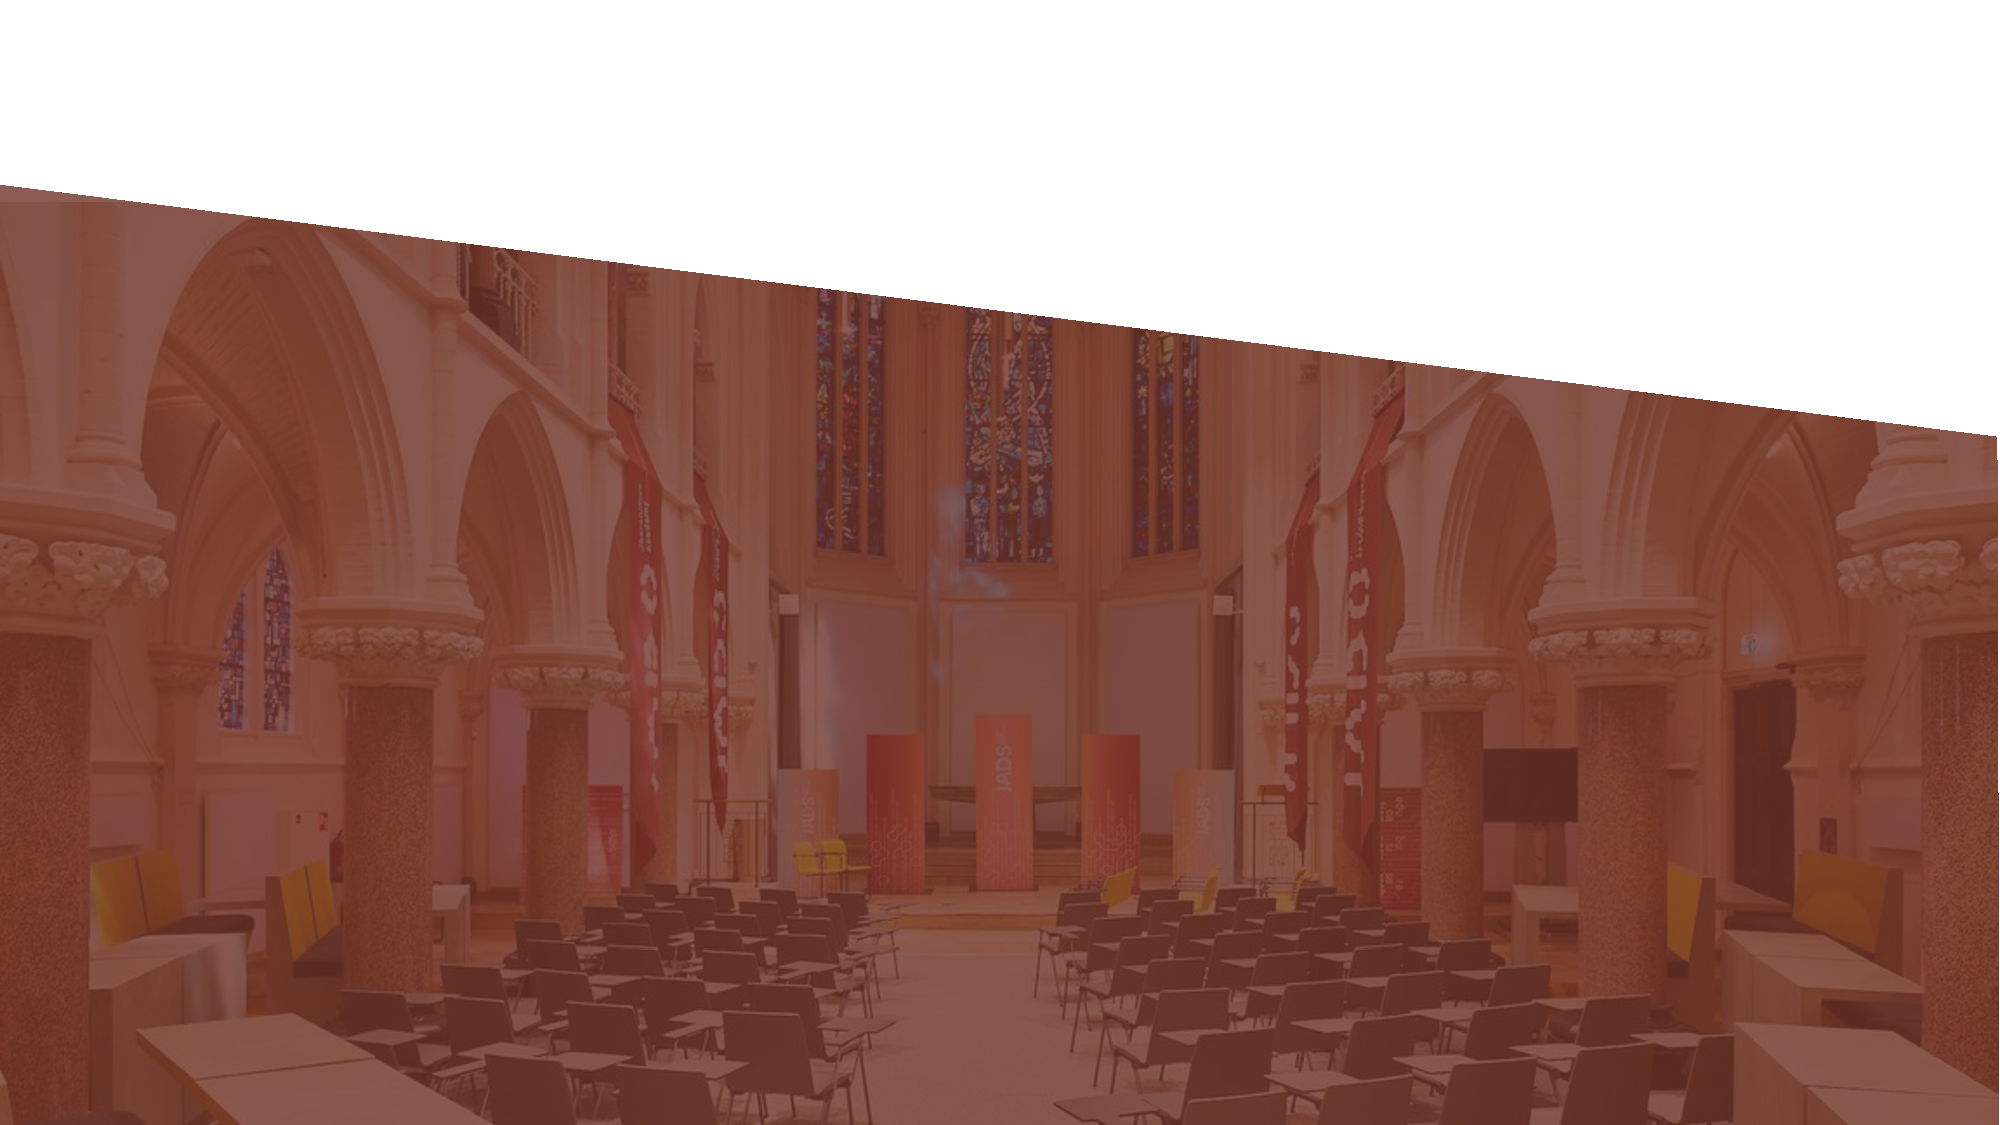
\includegraphics[width=\paperwidth]{template/figures/jads.pdf}};

\mbox{}
\vfill
\sffamily \Large \textcolor{white}{\placeanddate} \\

\end{titlepage}
\thispagestyle{empty}

\renewcommand*\contentsname{Table of contents}
{
\hypersetup{linkcolor=}
\setcounter{tocdepth}{2}
\tableofcontents
}

\section{Introduction}\label{sec-introduction}

TODO: topic, context (case and technique chosen), data available,
outline of the sections. TTPs follow the MITRE ATT\&CK taxonomy
\citep{attack}.

\section{Attack Investigation}\label{sec-attack-investigation}

TODO: investigation approach and how the incident was discovered in the
PCAP.

\subsection{Protocols and Mechanics}\label{sec-protocols}

TODO: protocol description.

\subsection{Incident Description}\label{sec-incident}

TODO: timeline, TTP table, affected assets, impact.

\begin{longtable}[]{@{}lllll@{}}
\caption{Chronological attack overview mapped to MITRE
ATT\&CK}\label{tbl-timeline}\tabularnewline
\toprule\noalign{}
Time & Observation & Evidence & ATT\&CK tactic & ATT\&CK technique \\
\midrule\noalign{}
\endfirsthead
\toprule\noalign{}
Time & Observation & Evidence & ATT\&CK tactic & ATT\&CK technique \\
\midrule\noalign{}
\endhead
\bottomrule\noalign{}
\endlastfoot
TODO & TODO & TODO & TODO & TODO \\
\end{longtable}

\subsection{Attack Mechanics}\label{sec-mechanics}

TODO: characteristics table or subsections.

\begin{longtable}[]{@{}
  >{\raggedright\arraybackslash}p{(\linewidth - 10\tabcolsep) * \real{0.1667}}
  >{\raggedright\arraybackslash}p{(\linewidth - 10\tabcolsep) * \real{0.1667}}
  >{\raggedright\arraybackslash}p{(\linewidth - 10\tabcolsep) * \real{0.1667}}
  >{\raggedright\arraybackslash}p{(\linewidth - 10\tabcolsep) * \real{0.1667}}
  >{\raggedright\arraybackslash}p{(\linewidth - 10\tabcolsep) * \real{0.1667}}
  >{\raggedright\arraybackslash}p{(\linewidth - 10\tabcolsep) * \real{0.1667}}@{}}
\caption{Attack characteristics and their detection
value}\label{tbl-characteristics}\tabularnewline
\toprule\noalign{}
\begin{minipage}[b]{\linewidth}\raggedright
Characteristic
\end{minipage} & \begin{minipage}[b]{\linewidth}\raggedright
Specificity
\end{minipage} & \begin{minipage}[b]{\linewidth}\raggedright
Benign overlap
\end{minipage} & \begin{minipage}[b]{\linewidth}\raggedright
Evasion difficulty
\end{minipage} & \begin{minipage}[b]{\linewidth}\raggedright
Automatable
\end{minipage} & \begin{minipage}[b]{\linewidth}\raggedright
Stage
\end{minipage} \\
\midrule\noalign{}
\endfirsthead
\toprule\noalign{}
\begin{minipage}[b]{\linewidth}\raggedright
Characteristic
\end{minipage} & \begin{minipage}[b]{\linewidth}\raggedright
Specificity
\end{minipage} & \begin{minipage}[b]{\linewidth}\raggedright
Benign overlap
\end{minipage} & \begin{minipage}[b]{\linewidth}\raggedright
Evasion difficulty
\end{minipage} & \begin{minipage}[b]{\linewidth}\raggedright
Automatable
\end{minipage} & \begin{minipage}[b]{\linewidth}\raggedright
Stage
\end{minipage} \\
\midrule\noalign{}
\endhead
\bottomrule\noalign{}
\endlastfoot
TODO & TODO & TODO & TODO & TODO & TODO \\
\end{longtable}

\section{Detection Method Development and
Evaluation}\label{sec-detection}

TODO: overview of the methods and how they map to the characteristics.

\subsection{Detection Method 1: {[}technique{]}}\label{sec-method-1}

TODO

\subsection{Detection Method 2 (optional)}\label{sec-method-2}

TODO

\section{Mitigation and Protection}\label{sec-mitigation}

TODO

\section{Discussion}\label{sec-discussion}

\subsection{Investigation}\label{investigation}

TODO

\subsection{Detection Method Development and
Evaluation}\label{detection-method-development-and-evaluation}

TODO

\subsection{Future Opportunities}\label{future-opportunities}

TODO

\section{Conclusion}\label{sec-conclusion}

TODO

\section*{References}\label{references}
\addcontentsline{toc}{section}{References}

\renewcommand{\bibsection}{}
\bibliography{references.bib}

\newpage
\appendix

\section*{Appendix A: Atomic Indicators of
Compromise}\label{appendix-a-atomic-indicators-of-compromise}
\addcontentsline{toc}{section}{Appendix A: Atomic Indicators of
Compromise}

\begin{landscape}

| Type | Value | Context | First seen |
|---|---|---|---|
| IP | TODO | TODO | TODO |
| Domain | TODO | TODO | TODO |

: Atomic indicators of compromise {#tbl-iocs}

\end{landscape}

\section*{Appendix B: Additional Figures and
Tables}\label{appendix-b-additional-figures-and-tables}
\addcontentsline{toc}{section}{Appendix B: Additional Figures and
Tables}

TODO





\end{document}
